\section{DBLP Dataset Analysis} 
\label{sec:dblp}

We studied the DBLP dataset which contains basic bibliographic information of publications from the computer science field. This data is freely available\footnote{\url{http://www.informatik.uni-trier.de/~ley/db/}} and contains highly relevant information about publication activity from the period of nearly fifty years, even though they are not complete. At the time we downloaded this dataset (July 2016), and after first pre-processing, it contained a total of $2988015$ publications. Further characteristics can be seen in Table \ref{tab:dblp}. 
\begin{table}[htbp]
  \centering
  \caption{DBLP dataset}
    \begin{tabular}{|l|r|} 
		\hline
    Total number of publications & 2988015 \\
    Total number of authors & 1622828 \\
    Mean papers per author & 5.113 \\
    Mean authors per paper & 2.895 \\
    \hline
    \end{tabular}%
  \label{tab:dblp}%
\end{table}%

Based on the co-authorship of authors, we constructed a social network where authors are linked if they co-authored a paper. The weight of the edge corresponds to the number of co-authored papers. Basic characteristics of this network and its maximal connected component are in Table \ref{tab:dblpcompo}.


\begin{table}[htbp]
  \centering
  \caption{DBLP network and its max. connected component}
	%\resizebox{0.8\columnwidth}{!}{
		\begin{tabular}{|l|rr|}
    \hline
          & $net$ & $max CC$\\
    \hline
    Total number of nodes & 1554772 & 1408331 \\
    Total number of edges & 6930545 & 6768108 \\
    Density & 5.73\mbox{\sc{e}-}06 & 6.83\mbox{\sc{e}-}06 \\
    Mean degree & 8.915 & 9.612 \\
    Number of connected components & 49459 & 1 \\
    Global clustering coefficient & 0.1749 & 0.1741 \\
    Mean local cluster coefficient & 0.7341 & 0.7217 \\
    Mean edge weight & 1.746 & 1.762 \\
    Number of communities (Louvain) &   -    & 422 \\
    \hline
    \end{tabular}%
		%}
  \label{tab:dblpcompo}%
\end{table}%

In additional pre-processing of the dataset, we set each publication a month which corresponded to the date of a conference or date of publication in a journal, respectively.  If the record in the DBPL did not contain the month of publication, we chose the month for a given year randomly. Furthermore, we assumed that the author existing in a given month is the author who had at least one publication in the month preceding the given month. In the next step, we dropped all publications that did not contain any already existing authors. For the rest of publications, we have identified the main author, who was the first existing author in the order of the co-authors of these publications.


The first objective of the experiment with the DBLP dataset was to discover what shape has the distribution of the number of publications depending on the number of co-authors of the main author. Figure \ref{fig:poisfit} shows the distribution for the first twenty values (i.e. up to $20$ co-authors) and cumulative distribution of all values (except for one publication with $286$ authors). This distribution is compared to a Poisson distribution with a $\lambda$ value equal to the average number of co-authors, which is $1.99$.


\begin{figure}[ht]
\centering
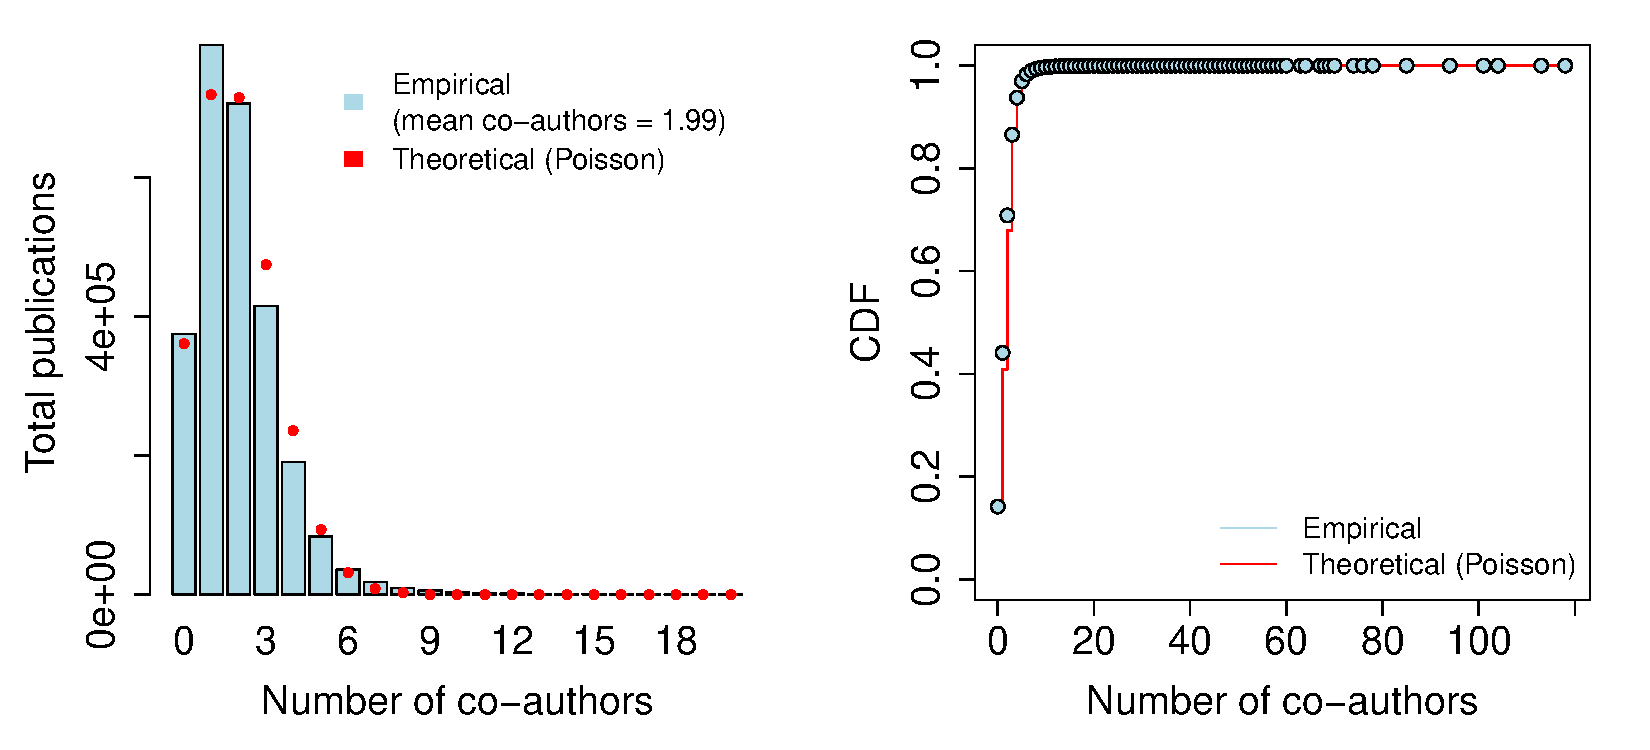
\includegraphics[width=\linewidth]{figures/poisfit}
  \caption{DBLP: Poisson distribution}\label{fig:poisfit}
\end{figure}

The second objective of the experiment was to find authors who are most often in the role of the main author of a publication. The results of this part of the experiment are to be understood only as an estimate based on the above-mentioned assumptions about the main author. Empirical distribution, together with the theoretical value of the Poisson distribution for the first fifteen authors with the highest number of publications in the role of the first author, is shown in Figure \ref{fig:top15}.

\begin{figure}[ht]
\centering
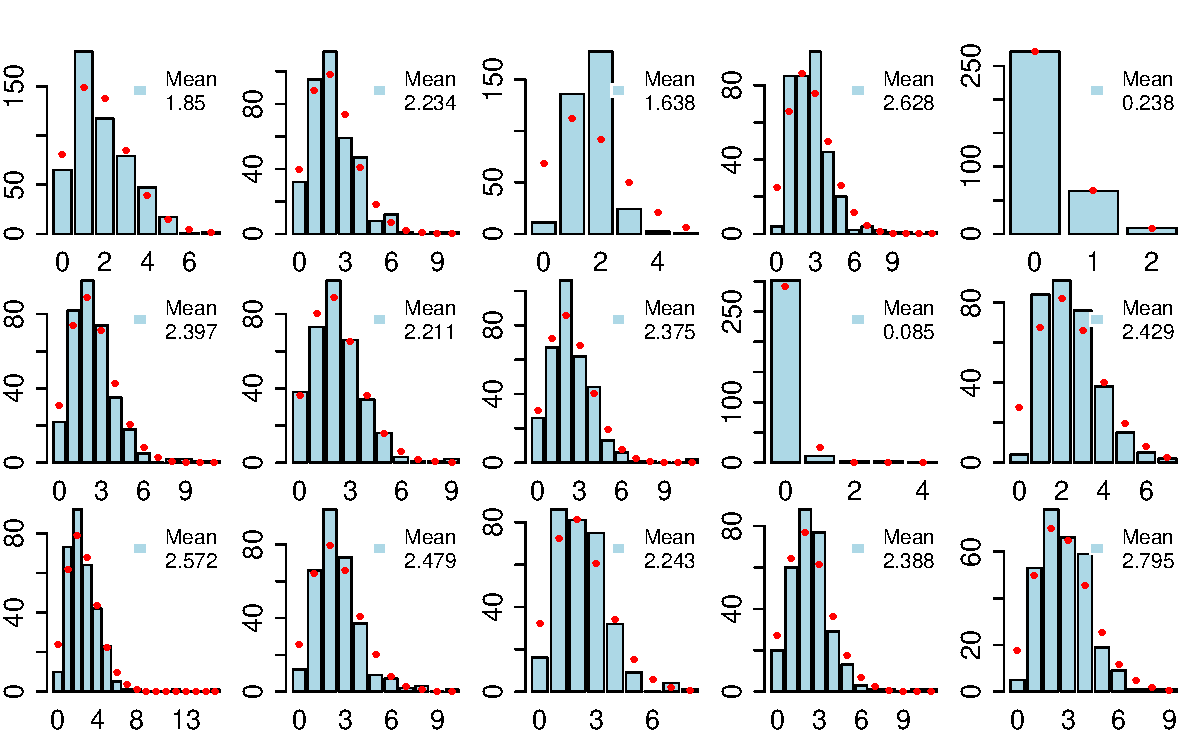
\includegraphics[width=\linewidth]{figures/proactive_coauthors_top15}
  \caption{Co-authors histograms for top 15 authors (by number of publications)}
	\label{fig:top15}
\end{figure}

\subsection{Hypothesis}
Results of the analysis of the DBLP dataset can not be easily generalized. However, experiments have shown quite clearly that the probability of a publication with a certain number of co-authors follows the Poisson distribution. If we extend thoughts about the main author by what kind and how many different co-authors he/she has, we may divide co-authors into three groups. In the first group are authors with whom the main author has previously published. In the second group are those who have previously published but not yet together with the main author. In the third group are new authors, i.e. those who have no previous publications. We can then formulate a hypothesis, based on which we define the new network model in the next part of the paper.

\bigbreak
\textbf{Hypothesis}
\begin{enumerate}
	\item The variables describing the number of co-authors in different groups are independent random variables.
  \item Just as the total number of co-authors, these variables follow Poisson distribution.
\end{enumerate}

In this paper, we are working with a co-authorship network, which is essentially a collaborative network. Therefore, the presented model can not be taken as a universal model. The model is primarily about a simple simulation of the development of collaborative networks inspired by analyzing the co-authorship network.
